\section{Algorithm}
\label{sec:layout}

The algorithm consists of two parts. First, the layout of schemas is generated; and then their outlines are computed based on the layout information.

\subsection{SchemaLine Layout}
\label{sub:schema-layout}
Besides compact and aesthetics, we set these requirements to the layout: 
\begin{enumerate}
	\item \textbf{Horizontal position}. Along the time axis, events should be placed exactly at when they happen whenever possible.
	\item \textbf{Relative order}. To improve the layout, events can be shifted horizontally; however, the their relative order must be maintained. 
	\item \textbf{Overlap free}. Events and schemas are not allowed to intersect each other.
\end{enumerate}

The layout algorithm consists of the following four steps (Fig.~\ref{fig:layout-overview}):
\begin{enumerate} 
	\item Order the schemas vertically such that the total number of shared events between neighboring schemas is maximized.
	\item For each schema, generate relative positions of its events -- satisfying the aforementioned requirements.
	\item Compact the schemas using the order computed in the first step.
	\item Position the remaining events that do not belong to any schemas. 
\end{enumerate}

\begin{figure}[ht]
\centering
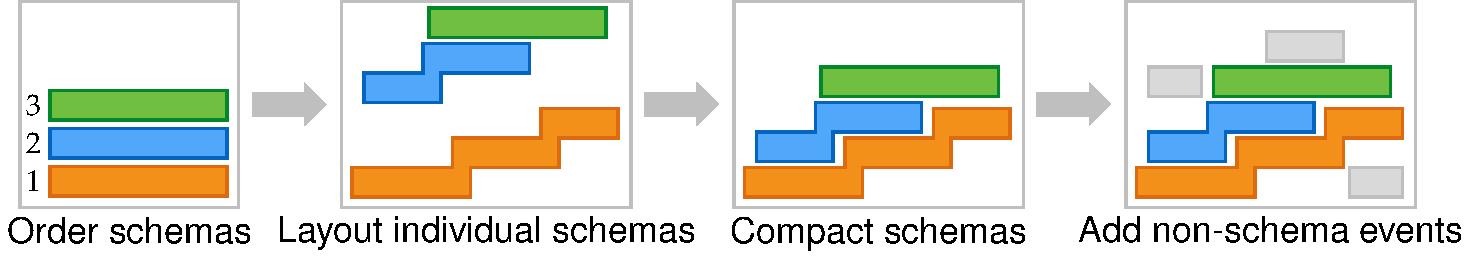
\includegraphics[width=\linewidth]{layout-overview}
\caption{SchemaLine layout algorithm. First, the order of all schemas is computed. Second, the layout of each schema is generated independently. Third, schemas are compacted following the computed order. Finally, events that do not belong to any schemas are added.}
\label{fig:layout-overview}
\end{figure}

\subsubsection{Order Schemas}
\label{sub:layout-order}
This step computes the order of schemas maximizing the total number of shared events between neighboring schemas.
We atextrmy a strategy that prioritizes pairing of schemas according to how many events they share. To do this, we map the problem to graph path finding as below. Given a set of schemata $S$, we create an undirected graph $G = (V,E)$, where each vertex $v_i$ represents a schema $s_i \in S$. The weight of an edge $e_{ij}$ is the number of events shared by schemata $s_i$ and $s_j$. Finding a schema order with the maximum number of shared nodes placed next to each other becomes finding a path with maximum weight connecting all vertices in $G$. This classic longest path finding problem is NP-hard. The number of schemata we plan to support is at most eight due to the limitation of the small number of colors that human can distinguish. Therefore, we simply use brute-forte algorithm to find the path.

\subsubsection{Layout Individual Schemas}
\label{sub:layout-schema}
The second step of the algorithm produces the layout of each schema. Events shared by multiple schemata are replicated for each of them; therefore, the layout of each schema can be generated independently. Events within a schema are sorted chronologically so that they can be added from left to right. The algorithm works by adding one event at a time: the new event will stay at the same horizontal level as the previous one if it can, otherwise it will move up one level. When a event $n_i$ has the same time as the previous $n_{i-1}$, it needs to be moved up one level because they must have the same x-coordinate. Otherwise, if $n_i$ intersects with $n_{i-1}$, an attempt is made to shift $n_{i-1}$ to the left to make space for $n_i$ as discussed below. If the shifting is successful, the event stays in that level; otherwise, the event needs to move up one level.

%\vspace{-4mm}
\paragraph*{Shifting Events}
To address the issues of scalability and efficient use of space, accuracy of the event position can be sacrificed. For each event, its $x$-coordinate is initially set at event time ($C1$). Then, events can be shifted horizontally to the left by a limited amount, to make room for events that are after it temporally. An event can be rendered at the non-accurate position scaled with its time. However, to keep the event close to the accurate position, we set the maximum distance that a event can shift to its width. As a result, the event still overlaps with its time point on the timeline and provides reasonable indication to viewers of its true position. When shifting, it is crucial to maintain the relative order between the shifting event and other events ($C2$). For example, if event $n_i$ was to the left of $n$ before the shifting, it should remain on the left afterwards. Another important condition is that there is no intersection with any other event after the shifting ($C3$). An illustration of this algorithm is shown in Fig.~\ref{fig:layout-schema-example}.

\subsubsection{Compact Schemas}
\label{sub:layout-compact}
In the third step, the algorithm stacks schemata in the order computed in the first step to produce a compact visualization. For example, if two schemata cover non-overlapping time ranges, they can be placed in the same level to save display space. 

Replicated events are connected using a light dashed line.

The group of schemata that share events is added to the SchemaLine first. Their relative ordering top to bottom is fixed and each schema is pushed towards the bottom as much as possible to save display space. After this, schemata without any shared event are added, again from bottom up to find the lowest level possible.

\begin{figure}[ht]
\centering
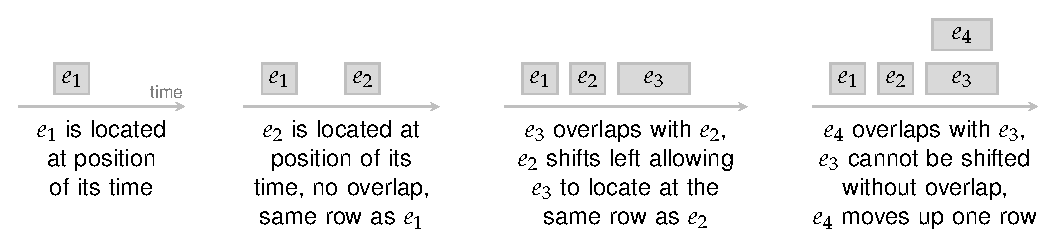
\includegraphics[width=\linewidth]{layout-example}
\caption{Schema layout algorithm. Four events \textrm{N1}, \textrm{N2}, \textrm{N3}, \textrm{N4} will be added to the schema in chronological order. \textrm{N1} is positioned at its accurate event time. \textrm{N2} can stay in the same level as \textrm{N1} because it does not intersect with \textrm{N1}. \textrm{N3} intersects with \textrm{N2} but the intersection width is small enough so that \textrm{N2} can be shifted to the left to let \textrm{N3} stay in the same level as well. However, \textrm{N4} needs to move up one level because the width of its intersection with \textrm{N3} is longer than that of \textrm{N1} and \textrm{N2}, i.e., they cannot be shifted.}
\label{fig:layout-schema-example}
\end{figure}

\subsubsection{Add Non-schema Events}
\label{sub:layout-non-schema}
This last step allocates events that do not belong to any schemata. Events are sorted chronologically so that they are added to the SchemaLine from left to right. The ideal $x$-position is the event time, but an event can be shifted as described in Section~\ref{sub:layout-schema}. An event always begins at the lowest level and moves upward until there is enough space for it: that is, until it does not intersect with any other schema or events after possible horizontal shifting. 

\subsection{SchemaLine Outline}
\label{sub:schema-outline}
In this section, we describe an algorithm to produce a polygonal outline covering all the event rectangles of a schema. We decided to use only horizontal and vertical line segments to keep the outline simple. The \emph{polygonal path} $P_n$ of a schema that contains $n$ event rectangles $R_1, R_2, ..., R_n$, ordered from left to right, is determined as follows:
\[
P_n=
\begin{cases}
R_1, & n=1 \\
P_{n-1} \oplus R_n, & n > 1
\end{cases},
\]
where $\oplus$ is an operator that merges a polygonal path and a rectangle into a new polygonal path. As described in the layout of individual schema (Section \ref{sub:layout-schema}), when a new event is added to an existing schema, it either has the same level as the previous event (Figure~\ref{fig:outline-right}) or one level higher (Figure~\ref{fig:outline-up}). To produce a nice path, two other special cases need to be considered as described in Figure~\ref{fig:outline-up-one} and Figure~\ref{fig:outline-up-two}.

\begin{figure}[ht]
	\centering
	\subcaptionbox{\label{fig:outline-right}\textrm{R3} is on the right side of the path.}{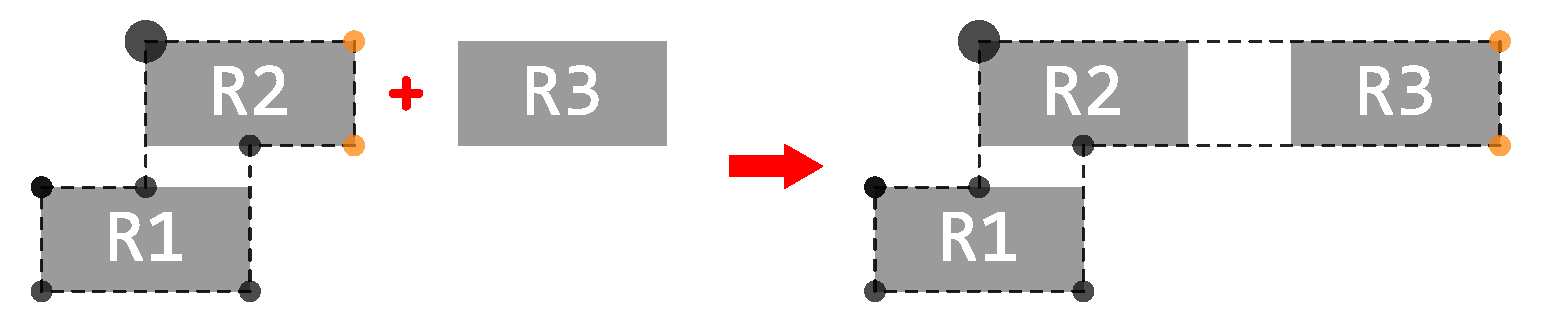
\includegraphics[width=0.8\columnwidth]{example-right}}
	\hfill
	\subcaptionbox{\label{fig:outline-up}\textrm{R3} is on top of the path.}{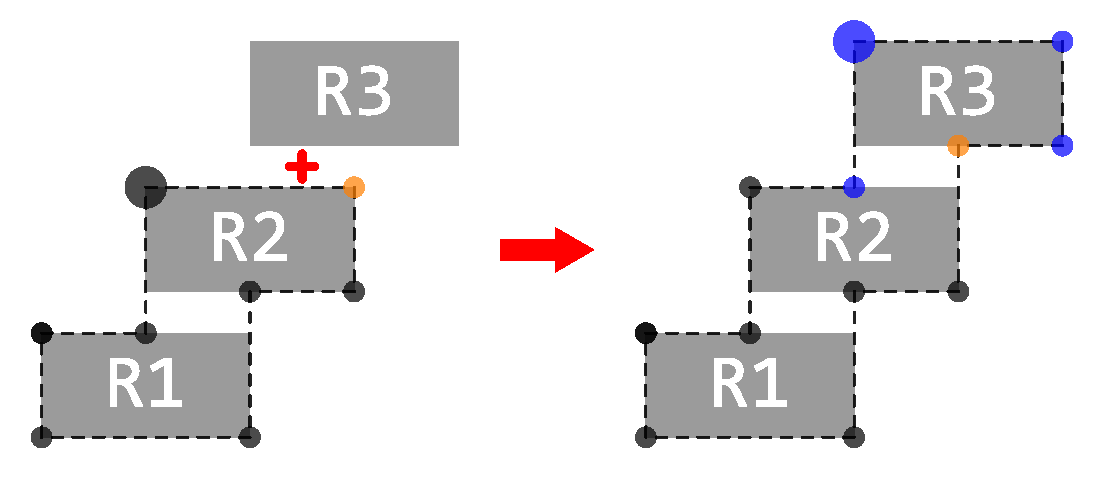
\includegraphics[width=0.55\columnwidth]{example-up}}
	\\
	\subcaptionbox{\label{fig:outline-up-one}Left-side of \textrm{R3} is a bit greater than left-side of \textrm{R2}.}[.4\linewidth]{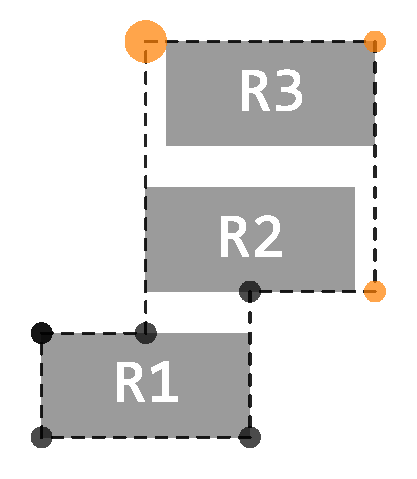
\includegraphics[width=0.25\columnwidth]{example-up-smoothing}}
	\hfill
	\subcaptionbox{\label{fig:outline-up-two}Right-side of \textrm{R3} is shorter than right-side of \textrm{R2}.}[.4\linewidth]{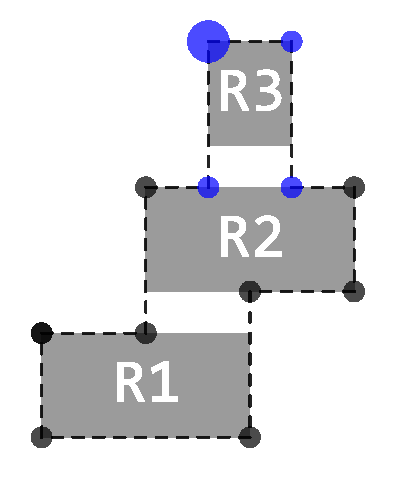
\includegraphics[width=0.24\columnwidth]{example-up-shorter}}
	\caption{Four cases when a new rectangle \textrm{R3} is appended to the polygonal path. A big circle indicates the pivot vertex of the path (top-left corner of the last rectangle). Orange circles indicate updated vertices, and blue circles indicate newly added vertices of the polygonal path.}
	\label{fig:outline}
\end{figure}

After producing a rectilinear path, the bends are made rounded (Fig.~\ref{fig:teaser}). The path is filled with the same stroke color but less transparency to make the border stand out with a darker hue. The beginning of the path does not have the border to indicate that the path is open on that side and the reader should follow this direction. 